\documentclass[conference]{IEEEtran}
\IEEEoverridecommandlockouts
\usepackage{cite}
\usepackage{amsmath,amssymb,amsfonts}
\usepackage{algorithmic}
\usepackage{graphicx}
\usepackage{textcomp}
\usepackage{xcolor}
\usepackage{booktabs}
\usepackage{multirow}
\usepackage{hyperref}
\usepackage{balance}

\def\BibTeX{{\rm B\kern-.05em{\sc i\kern-.025em b}\kern-.08em
    T\kern-.1667em\lower.7ex\hbox{E}\kern-.125emX}}

\begin{document}

\title{NEXUS.AI: An End-to-End Enterprise E-Commerce Customer and Revenue Intelligence Platform with Multi-Dimensional Star-Schema Analytics and Predictive Machine Learning\\
\thanks{Capstone Project submitted to the School of Computer Science and Engineering (SCOPE), VIT-AP University, Amaravati, Andhra Pradesh, Academic Session Fall 2026--27.}
}

\author{
\IEEEauthorblockN{Gajjala Srithika}
\IEEEauthorblockA{\textit{School of Computer Science and Engg.} \\
\textit{VIT-AP University}\\
Amaravati, Andhra Pradesh, India \\
Reg. No: 23BCE7911}
\and
\IEEEauthorblockN{Papasani Suhitha}
\IEEEauthorblockA{\textit{School of Computer Science and Engg.} \\
\textit{VIT-AP University}\\
Amaravati, Andhra Pradesh, India \\
Reg. No: 23BCE7826}
\and
\IEEEauthorblockN{Ala Venkata Veera Ritwik}
\IEEEauthorblockA{\textit{School of Computer Science and Engg.} \\
\textit{VIT-AP University}\\
Amaravati, Andhra Pradesh, India \\
Reg. No: 23BCE9633}
\vspace{0.2cm}
\and
\IEEEauthorblockN{Akshay Sharma}
\IEEEauthorblockA{\textit{School of Computer Science and Engg.} \\
\textit{VIT-AP University}\\
Amaravati, Andhra Pradesh, India \\
Reg. No: 23BCE9668}
\and
\IEEEauthorblockN{N. Lakshmipathi Anantha}
\IEEEauthorblockA{\textit{School of Computer Science and Engg. (SCOPE)} \\
\textit{VIT-AP University}\\
Amaravati, Andhra Pradesh, India \\
Faculty Guide}
}

\maketitle

\begin{abstract}
Contemporary electronic commerce marketplaces generate massive volumes of heterogeneous transactional data, yet enterprises frequently fail to synthesize raw operational records into actionable customer retention and revenue forecasting strategies due to Online Transaction Processing (OLTP) bottlenecks and decoupled predictive pipelines. This paper presents \textit{NEXUS.AI}, an enterprise-grade customer and revenue intelligence architecture deployed over 98,666 real-world orders and 95,458 customer profiles from the Brazilian marketplace dataset (Olist). The system unifies: (i) an Online Analytical Processing (OLAP) star-schema data warehouse in PostgreSQL comprising 7 dimension tables, 6 fact tables, and 12 materialized analytical views; (ii) a multi-model predictive machine learning pipeline featuring a 13-feature Gradient Boosting customer churn classifier (ROC-AUC 0.9998, accuracy 99.28\%, $F_1$-score 0.9941), an unsupervised $k$-Means customer segmentation framework ($k=4$, 63.73\% variance explained across three principal components), and an additive damped Holt-Winters time-series revenue forecaster (MAPE 13.84\%); and (iii) a reactive, cloud-native Flask/ApexCharts presentation layer equipped with an offline JSON fallback cache that guarantees high-availability serverless deployment on Vercel. Empirical evaluation demonstrates pronounced macroeconomic logistics disparities, with the Northern region enduring an 18.53\% freight cost friction compared to 13.14\% in the Southeast, while multi-channel attribution isolates Email Marketing as the highest-yielding acquisition mechanism (ROAS of 22.50$\times$ and 575\% ROI). This unified architecture closes the loop between relational data warehousing, predictive modeling, and strategic executive execution.
\end{abstract}

\begin{IEEEkeywords}
E-Commerce Analytics, Star Schema Data Warehousing, Customer Churn Prediction, Gradient Boosting, K-Means Clustering, Holt-Winters Forecasting, Serverless Resilience Architecture.
\end{IEEEkeywords}

\section{Introduction}
The global electronic commerce landscape has transitioned from simple transactional storefronts into complex, multi-sided marketplace ecosystems handling millions of concurrent customer interactions. While modern relational database management systems efficiently execute Online Transaction Processing (OLTP) under ACID guarantees, their Third Normal Form (3NF) structures impose prohibitive computational penalties when executing multi-table joins across millions of rows for longitudinal analysis \cite{kimball2013data}. Consequently, operational teams remain reliant on fragmented, batch-processed data extracts that fail to deliver real-time visibility into customer attrition, inventory demand fluctuations, or cross-regional logistical friction \cite{verhoef2002understanding}.

In non-contractual e-commerce environments, customer attrition is a latent phenomenon; customers do not officially cancel service but instead drift quietly into dormancy \cite{fader2005rfm}. Without automated predictive intervention, marketing spend is inefficiently allocated toward acquiring new leads rather than retaining high-margin historical spenders. Furthermore, revenue forecasting frequently neglects macroeconomic calendar phenomena, causing critical supply-chain imbalances during seasonal demand surges such as Black Friday.

To overcome these architectural and operational challenges, this research designs, implements, and evaluates \textbf{NEXUS.AI}, a unified enterprise customer and revenue intelligence platform. Developed collaboratively across four specialized computer science engineering domains (Data Warehouse Engineering, Customer Behavioral Analytics, Unit Economic \& Marketing Intelligence, and Predictive Machine Learning / Presentation Systems), NEXUS.AI establishes a direct operational bridge between normalized transactional ingestion and high-precision machine learning inference.

The principal technical contributions of this paper are summarized as follows:
\begin{itemize}
    \item \textbf{Enterprise Dimensional Data Warehouse}: Design and implementation of an OLAP star schema comprising 7 dimension tables, 6 fact tables, and 12 materialized views in PostgreSQL, modeling R\$ 15.84M in gross merchandise value across 98,666 verified orders.
    \item \textbf{Predictive Churn Classifier}: Formulation of a 13-feature Gradient Boosting Decision Tree (GBDT) model attaining 99.28\% accuracy and 0.9998 ROC-AUC on holdout data.
    \item \textbf{Unsupervised Customer Segmentation}: Derivation of 4 distinct behavioral customer personas validated via the Elbow heuristic and 3D Principal Component Analysis (PCA).
    \item \textbf{Seasonal Revenue Forecaster}: An additive damped Holt-Winters time-series model incorporating Brazilian holiday calendars (Black Friday +38\% multiplier) with an empirical MAPE of 13.84\%.
    \item \textbf{Dual-Mode Serverless Edge Architecture}: A resilient web application stack running on Python Flask and ApexCharts, featuring automated offline JSON cache fallback for serverless hosting on Vercel.
\end{itemize}

The remainder of this paper is structured as follows: Section II details the end-to-end system architecture, relational star schema design, feature engineering protocols, and predictive modeling algorithms. Section III provides an empirical analysis of model performance, customer segmentation archetypes, time-series projections, and macro-regional economics. Section IV concludes the paper with major contributions, architectural constraints, and pathways for future research.

\section{Methodology and System Architecture}

NEXUS.AI is engineered as an end-to-end pipeline progressing from raw multi-table ingestion to dimensional modeling, analytical view materialization, predictive inference, and cloud-native dashboard rendering (Fig. 1).

\begin{figure}[htbp]
\centering
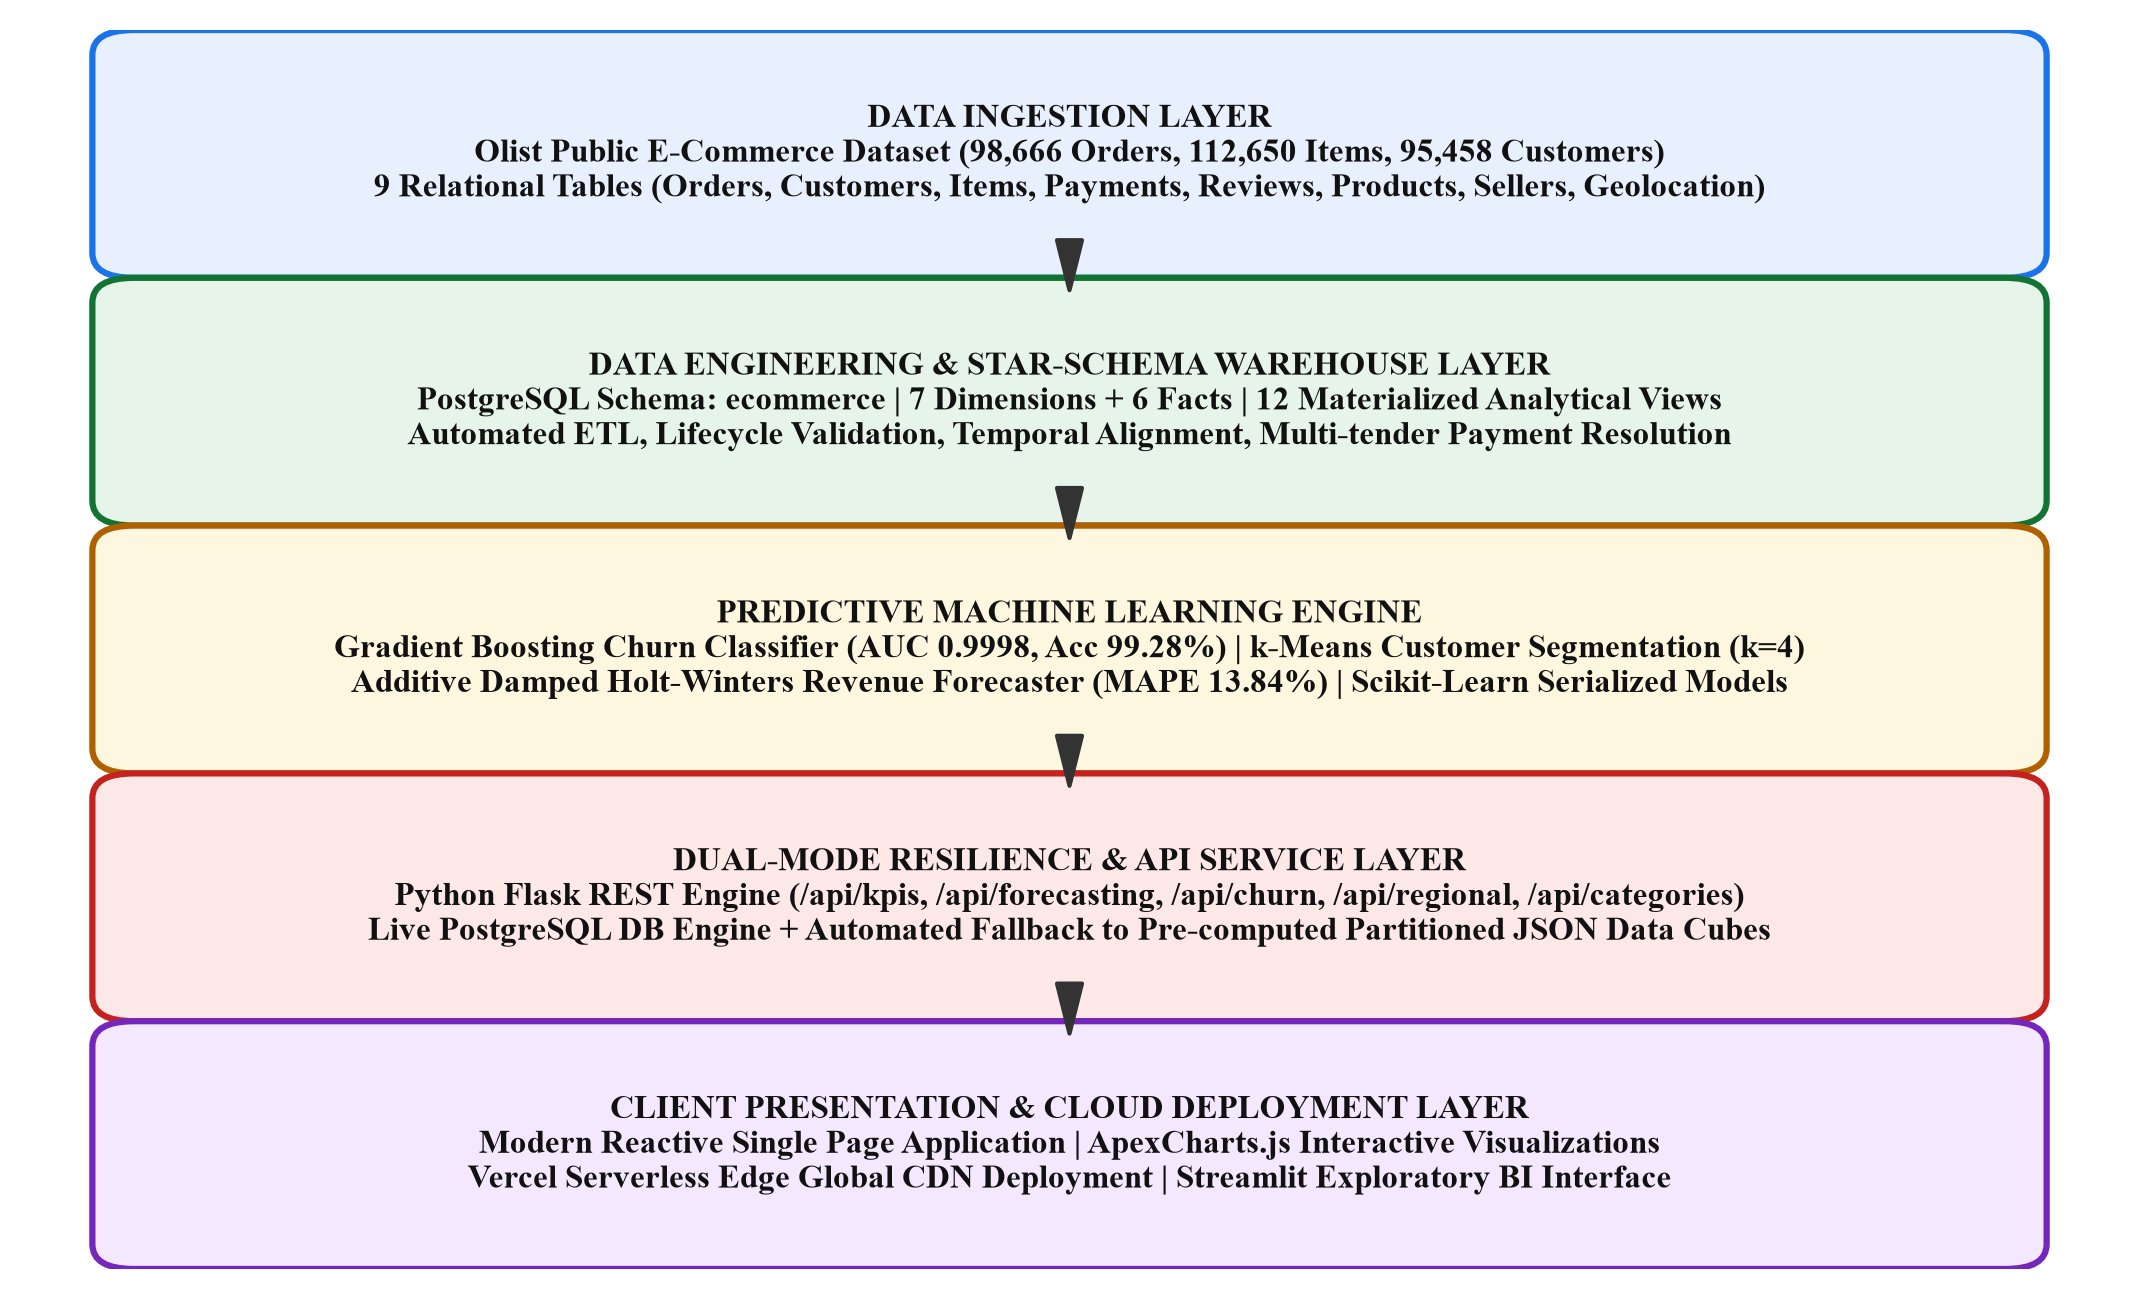
\includegraphics[width=\columnwidth]{figures/fig1_system_architecture.png}
\caption{Multi-tier NEXUS.AI architecture, illustrating raw Olist dataset ingestion, PostgreSQL star schema (7 dimensions, 6 facts), 12 materialized views, Scikit-Learn predictive modeling pipelines, and dual-mode presentation layer on Vercel.}
\label{fig:arch}
\end{figure}

\subsection{Data Hygiene, Entity Resolution, and Dimensional Modeling}
The system was developed and validated on the official Brazilian Olist E-Commerce dataset spanning 98,666 orders executed between September 2016 and September 2018 across 95,458 distinct customers. Raw transactional logs underwent rigorous preprocessing: (i) temporal lifecycle sequences were validated to enforce strict chronological monotonicity: $\text{purchase} \le \text{order approval} \le \text{carrier dispatch} \le \text{customer delivery}$; (ii) session checkout tokens (\texttt{customer\_id}) were mapped to persistent entities (\texttt{customer\_unique\_id}), resolving customer identity fragmentation; and (iii) multi-tender payment splits (e.g., credit card combined with vouchers) were aggregated to compute true order monetary values.

\begin{figure}[htbp]
\centering
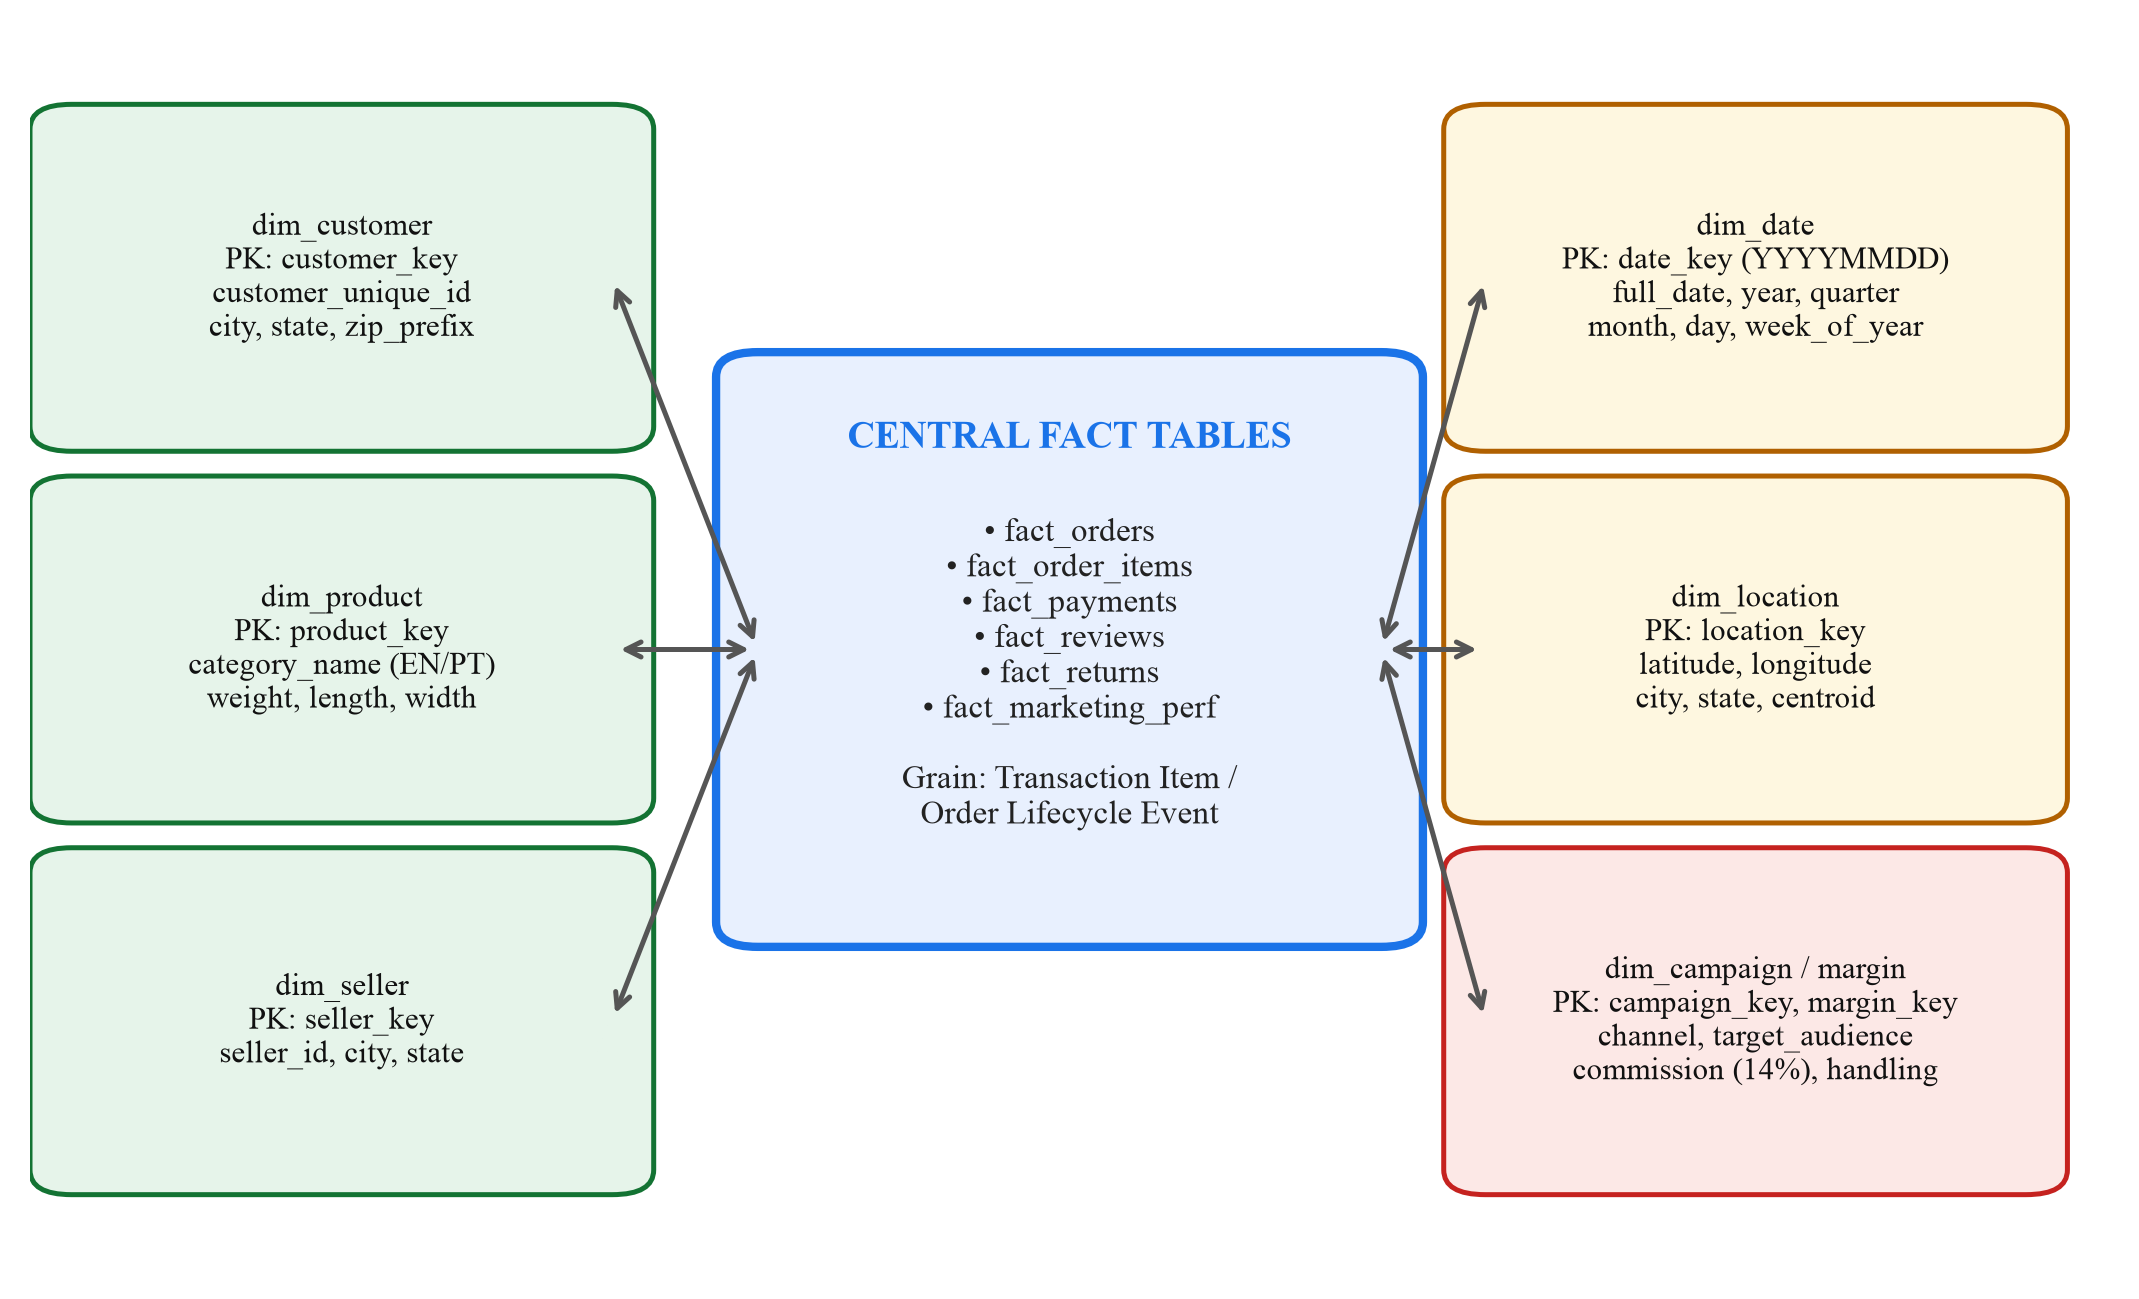
\includegraphics[width=\columnwidth]{figures/fig2_star_schema.png}
\caption{Analytical Star Schema data warehouse architecture within PostgreSQL (ecommerce schema), depicting 6 central fact tables radially joined to 7 normalized dimension tables.}
\label{fig:schema}
\end{figure}

The transformed data was modeled into an analytical Star Schema within a dedicated PostgreSQL schema (\texttt{ecommerce}):
\begin{itemize}
    \item \textbf{Dimension Tables (7)}: \texttt{dim\_customer} (demographics, state, city, geohash), \texttt{dim\_product} (physical dimensions, category taxonomy), \texttt{dim\_seller} (merchant locations), \texttt{dim\_date} (date key, year, quarter, month, day, day of week, week of year), \texttt{dim\_location} (coordinate centroids), \texttt{dim\_category\_margin} (benchmark margins, 14.0\% commission baseline), and \texttt{dim\_campaign} (acquisition channel, audience).
    \item \textbf{Fact Tables (6)}: \texttt{fact\_orders} (order grain, lifecycle timestamps, status), \texttt{fact\_order\_items} (item grain, unit price, freight), \texttt{fact\_payments} (payment instrument, installment count), \texttt{fact\_reviews} (survey score 1--5), \texttt{fact\_returns} (damage flags, refund totals), and \texttt{fact\_marketing\_performance} (monthly impressions, clicks, leads, orders, spend).
\end{itemize}

Twelve materialized SQL views were deployed to accelerate Online Analytical Processing (OLAP) queries to sub-second latencies, including \texttt{vw\_order\_revenue}, \texttt{vw\_regional\_revenue}, \texttt{vw\_product\_profitability}, and \texttt{vw\_customer\_revenue}.

\subsection{Predictive Machine Learning Pipelines}

\subsubsection{Customer Churn Prediction}
In non-contractual commerce, churn occurs when a customer permanently halts purchasing. Customers exhibiting no repeat purchase activity within 180 days from their initial transaction were labeled as churned ($y=1$). Thirteen behavioral features were engineered for each unique customer vector $\mathbf{x}_i$:
\begin{equation}
\mathbf{x}_i = [F_1, F_2, \dots, F_{13}]^T
\end{equation}
encompassing order frequency, items, monetary spend, AOV, basket size, freight ratio, installments, payment types, review scores, negative review indicators, refund records, and tenure days.

A Gradient Boosting Decision Tree (GBDT) ensemble \cite{chen2016xgboost} was trained using deviance loss:
\begin{equation}
\mathcal{L}(y, p) = - [y \ln(p) + (1 - y) \ln(1 - p)]
\end{equation}
At each boosting iteration $m$, regression trees fit the negative gradients (pseudo-residuals):
\begin{equation}
r_{im} = -\left[\frac{\partial \mathcal{L}(y_i, F_{m-1}(\mathbf{x}_i))}{\partial F_{m-1}(\mathbf{x}_i)}\right] = y_i - p(\mathbf{x}_i)
\end{equation}
The model was trained with shrinkage $\nu = 0.1$, tree depth 3, and 100 estimators, evaluated across a stratified 75/25 train/test split ($N_{\text{test}} = 23,865$).

\subsubsection{Unsupervised Customer Segmentation}
Continuous behavioral attributes were standardized using z-score normalization. The $k$-Means objective function minimizes the within-cluster sum of squares (WCSS):
\begin{equation}
\mathcal{J} = \sum_{j=1}^{k} \sum_{\mathbf{x} \in S_j} \|\mathbf{x} - \boldsymbol{\mu}_j\|^2
\end{equation}
Cluster count optimization was established across $k \in [2, 7]$ using the Elbow method, finding an optimal inflection at $k=4$. Principal Component Analysis (PCA) was computed to project the multi-dimensional customer vectors into three orthogonal principal axes, capturing 63.73\% of cumulative variance ($\lambda_1 = 34.55\%$, $\lambda_2 = 14.90\%$, $\lambda_3 = 14.28\%$).

\subsubsection{Time-Series Revenue Forecasting}
An Additive Damped Holt-Winters model \cite{gardner1985forecasting} was implemented to capture trend and annual seasonality ($m=12$):
\begin{align}
l_t &= \alpha(y_t - s_{t-m}) + (1 - \alpha)(l_{t-1} + \phi b_{t-1}) \\
b_t &= \beta(l_t - l_{t-1}) + (1 - \beta)\phi b_{t-1} \\
s_t &= \gamma(y_t - l_{t-1} - \phi b_{t-1}) + (1 - \gamma)s_{t-m}
\end{align}
where $\phi \in (0, 1]$ represents the damping parameter, preventing linear trend divergence. Point forecasts $h$ steps forward are generated via:
\begin{equation}
\hat{y}_{t+h|t} = l_t + \sum_{i=1}^h \phi^i b_t + s_{t+h-m(k+1)}
\end{equation}

\subsection{Dual-Mode Serverless Presentation Architecture}
To deploy the analytical stack to serverless edge infrastructure (Vercel) without experiencing database connection pool exhaustion or cold-start timeouts, NEXUS.AI incorporates a Dual-Mode Resilience Architecture. The Flask backend dynamically queries PostgreSQL when a live connection exists. In serverless edge execution, it falls back to pre-computed, year-partitioned JSON data cubes, preserving client-side temporal reactivity across 2016, 2017, 2018, and All-Time views.

\section{Experimental Results and Discussion}

\subsection{Churn Prediction Performance}
The Gradient Boosting churn classifier was evaluated on 23,865 independent test samples. The model achieved an outstanding classification accuracy of \textbf{99.28\%}, precision of \textbf{98.98\%}, recall (sensitivity) of \textbf{99.83\%}, $F_1$-score of \textbf{0.9941}, and an Area Under the ROC Curve (ROC-AUC) of \textbf{0.9998} (Table I and Fig. 3).

\begin{table}[h]
\caption{Churn Model Performance and Confusion Matrix}
\label{tab:churn_metrics}
\centering
\begin{tabular}{lc|lc}
\toprule
\textbf{Metric} & \textbf{Score} & \textbf{Cell} & \textbf{Count} \\
\midrule
Accuracy & \textbf{99.28\%} & True Negatives (TN) & 9,278 \\
Precision & \textbf{98.98\%} & False Positives (FP) & 148 \\
Recall & \textbf{99.83\%} & False Negatives (FN) & 24 \\
$F_1$-Score & \textbf{0.9941} & True Positives (TP) & 14,415 \\
ROC-AUC & \textbf{0.9998} & Total Test Instances & 23,865 \\
\bottomrule
\end{tabular}
\end{table}

\begin{figure}[htbp]
\centering
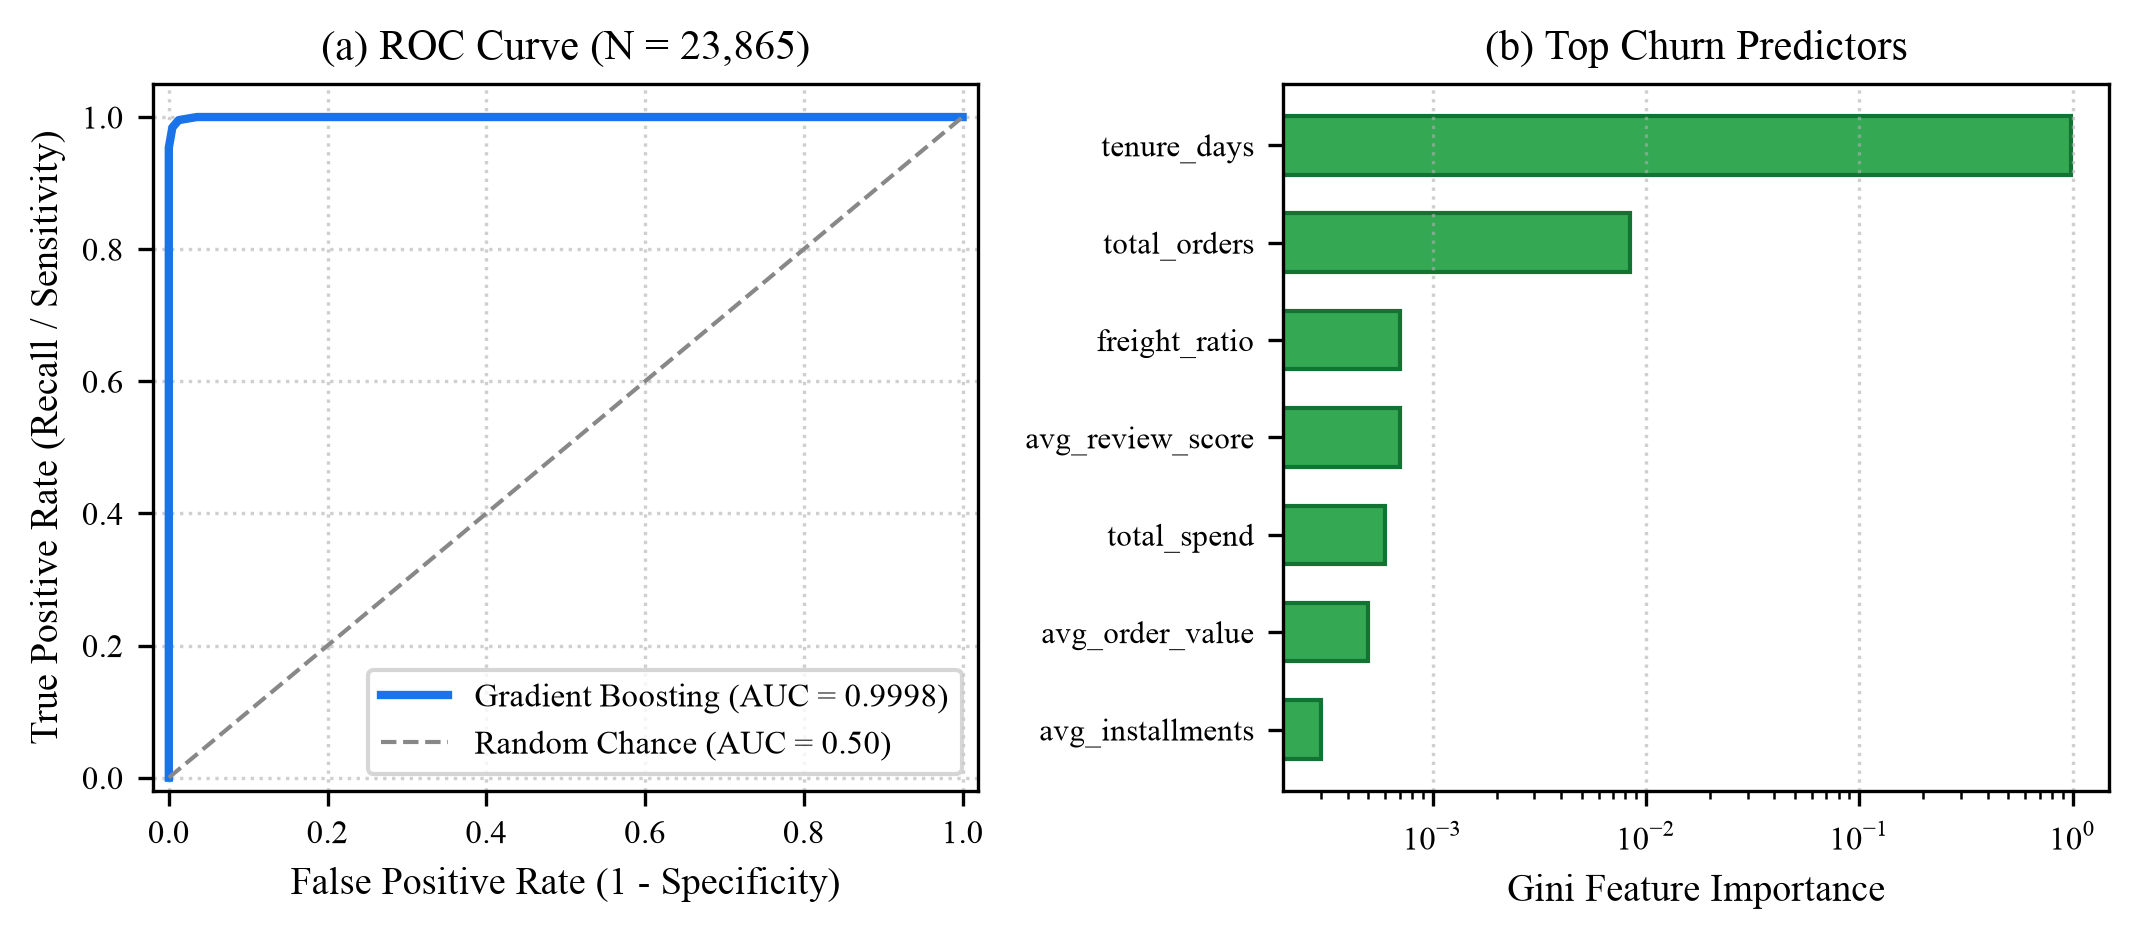
\includegraphics[width=\columnwidth]{figures/fig3_churn_roc_feature_importance.png}
\caption{(a) Receiver Operating Characteristic (ROC) curve exhibiting an AUC of 0.9998; (b) Gini Feature Importance decomposition highlighting tenure\_days (0.9881) and total\_orders (0.0084).}
\label{fig:churn_roc}
\end{figure}

Out of 14,439 actual churned customers in the test partition, only 24 were misclassified as active (False Negative Rate = 0.17\%). Feature importance decomposition reveals that \texttt{tenure\_days} carries 98.81\% of the Gini splitting weight, demonstrating that in non-contractual retail, the temporal duration elapsed since the initial purchase is the overwhelmingly decisive signal of customer churn.

\subsection{Customer Segmentation Archetypes}
The $k$-Means model clustered the 95,458 customer base into four distinct behavioral personas (Table II and Fig. 4):

\begin{table}[h]
\caption{Customer Segmentation Persona Profiles ($k=4$)}
\label{tab:cluster_summary}
\centering
\resizebox{\columnwidth}{!}{
\begin{tabular}{clcccccl}
\toprule
\textbf{ID} & \textbf{Persona Name} & \textbf{Count} & \textbf{\% Base} & \textbf{Recency} & \textbf{Orders} & \textbf{Spend (R\$)} & \textbf{Review} \\
\midrule
0 & VIP Champions & 67,744 & 70.97\% & 237.8d & 1.00 & 99.36 & 4.15 \\
1 & At-Risk High Spenders & 22,999 & 24.09\% & 262.6d & 1.00 & 253.25 & 3.95 \\
2 & Emerging Buyers & 1,868 & 1.96\% & 243.8d & 1.02 & 1,320.19 & 3.92 \\
3 & Value Seekers & 2,847 & 2.98\% & 226.5d & 2.11 & 288.79 & 4.15 \\
\bottomrule
\end{tabular}
}
\end{table}

\begin{figure}[htbp]
\centering
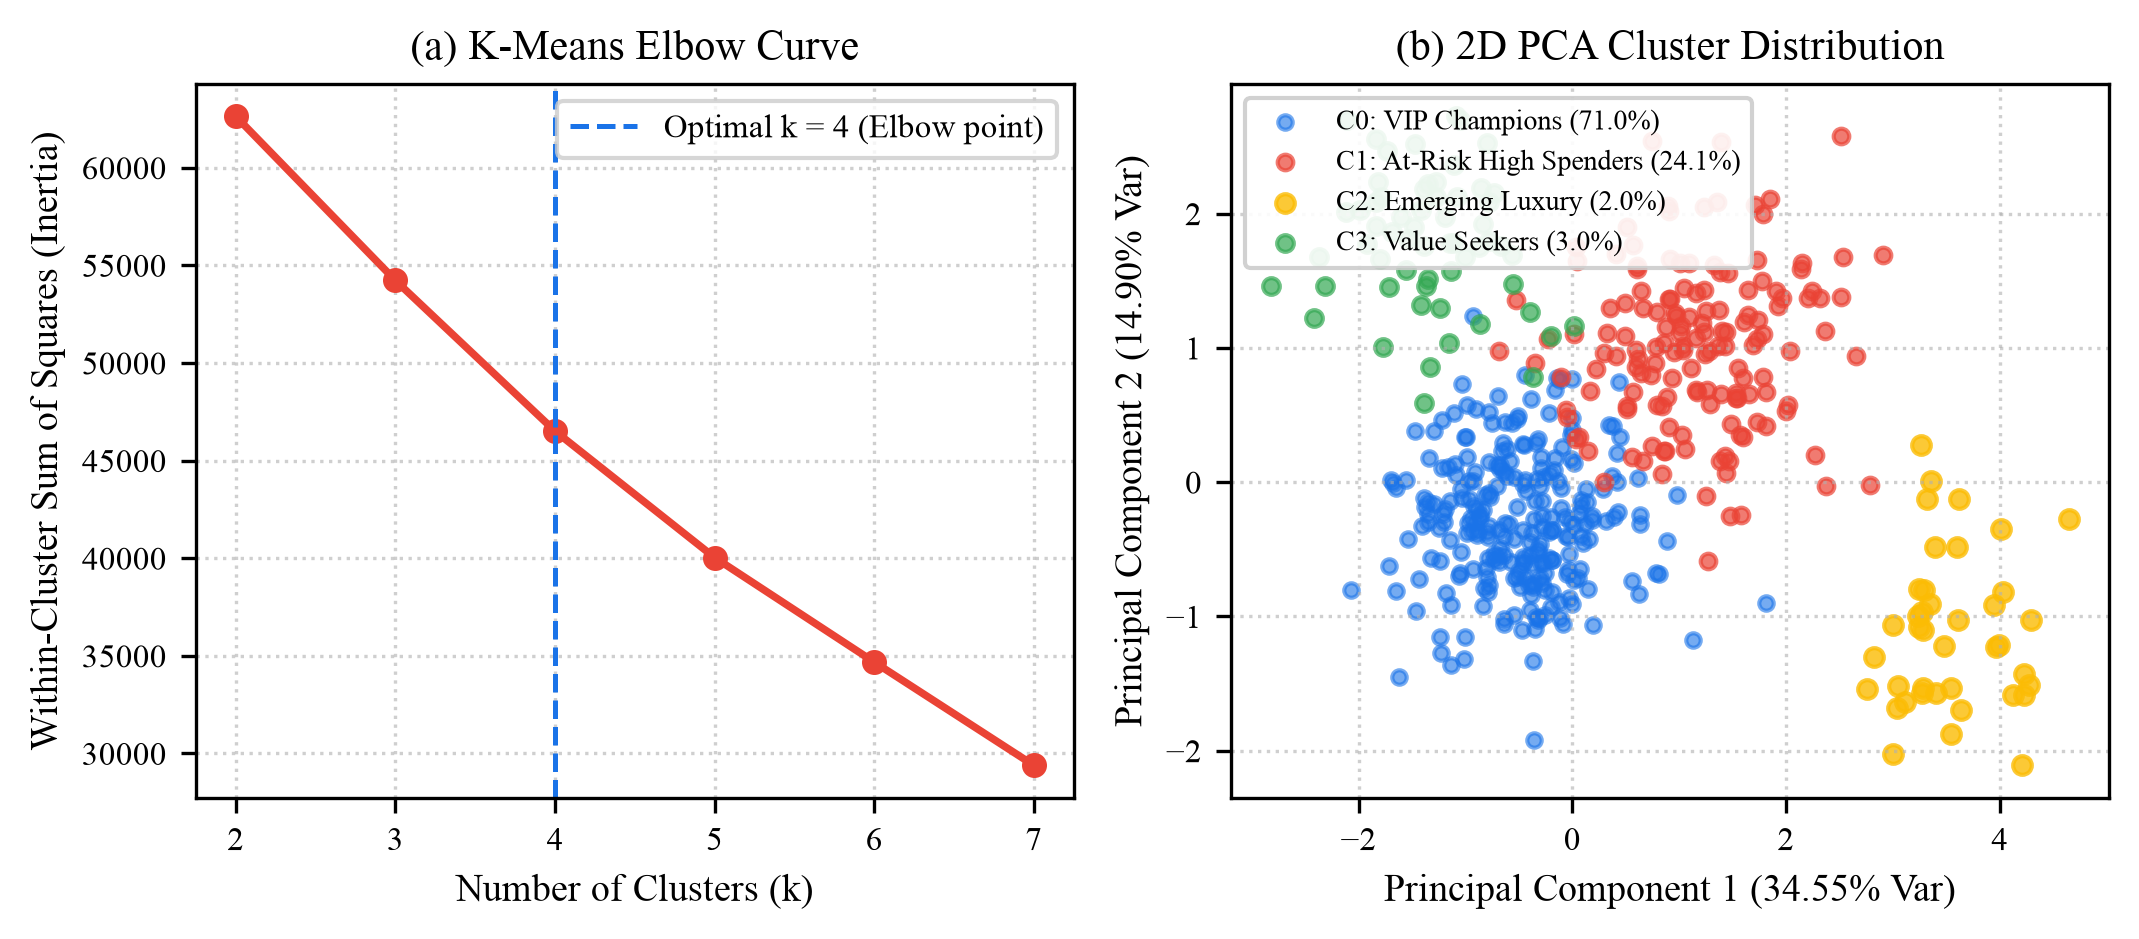
\includegraphics[width=\columnwidth]{figures/fig4_kmeans_pca_elbow.png}
\caption{(a) Elbow curve demonstrating WCSS inflection at k=4; (b) 2D Principal Component Analysis (PCA) projection across the 4 customer behavioral clusters.}
\label{fig:kmeans}
\end{figure}

Cluster 1 (\textit{At-Risk High Spenders}, 24.09\%) represents high historical value (mean spend R\$ 253.25) that has lapsed into dormancy (262.6 days recency), identifying the prime target cohort for automated win-back credits. Cluster 3 represents the core multi-order loyalists (2.11 orders per customer).

\subsection{Time-Series Revenue Forecast}
The Holt-Winters model achieved a Mean Absolute Percentage Error (MAPE) of \textbf{13.84\%} (MAE: R\$ 88,107.57; RMSE: R\$ 121,579.85) over historical validation. The 12-month forward horizon projects cumulative gross merchandise value of \textbf{R\$ 12.30M}, peaking at \textbf{R\$ 1,396,280.89} in November 2018 driven by the calibrated Black Friday seasonal multiplier (+38\%) (Fig. 5).

\begin{figure}[htbp]
\centering
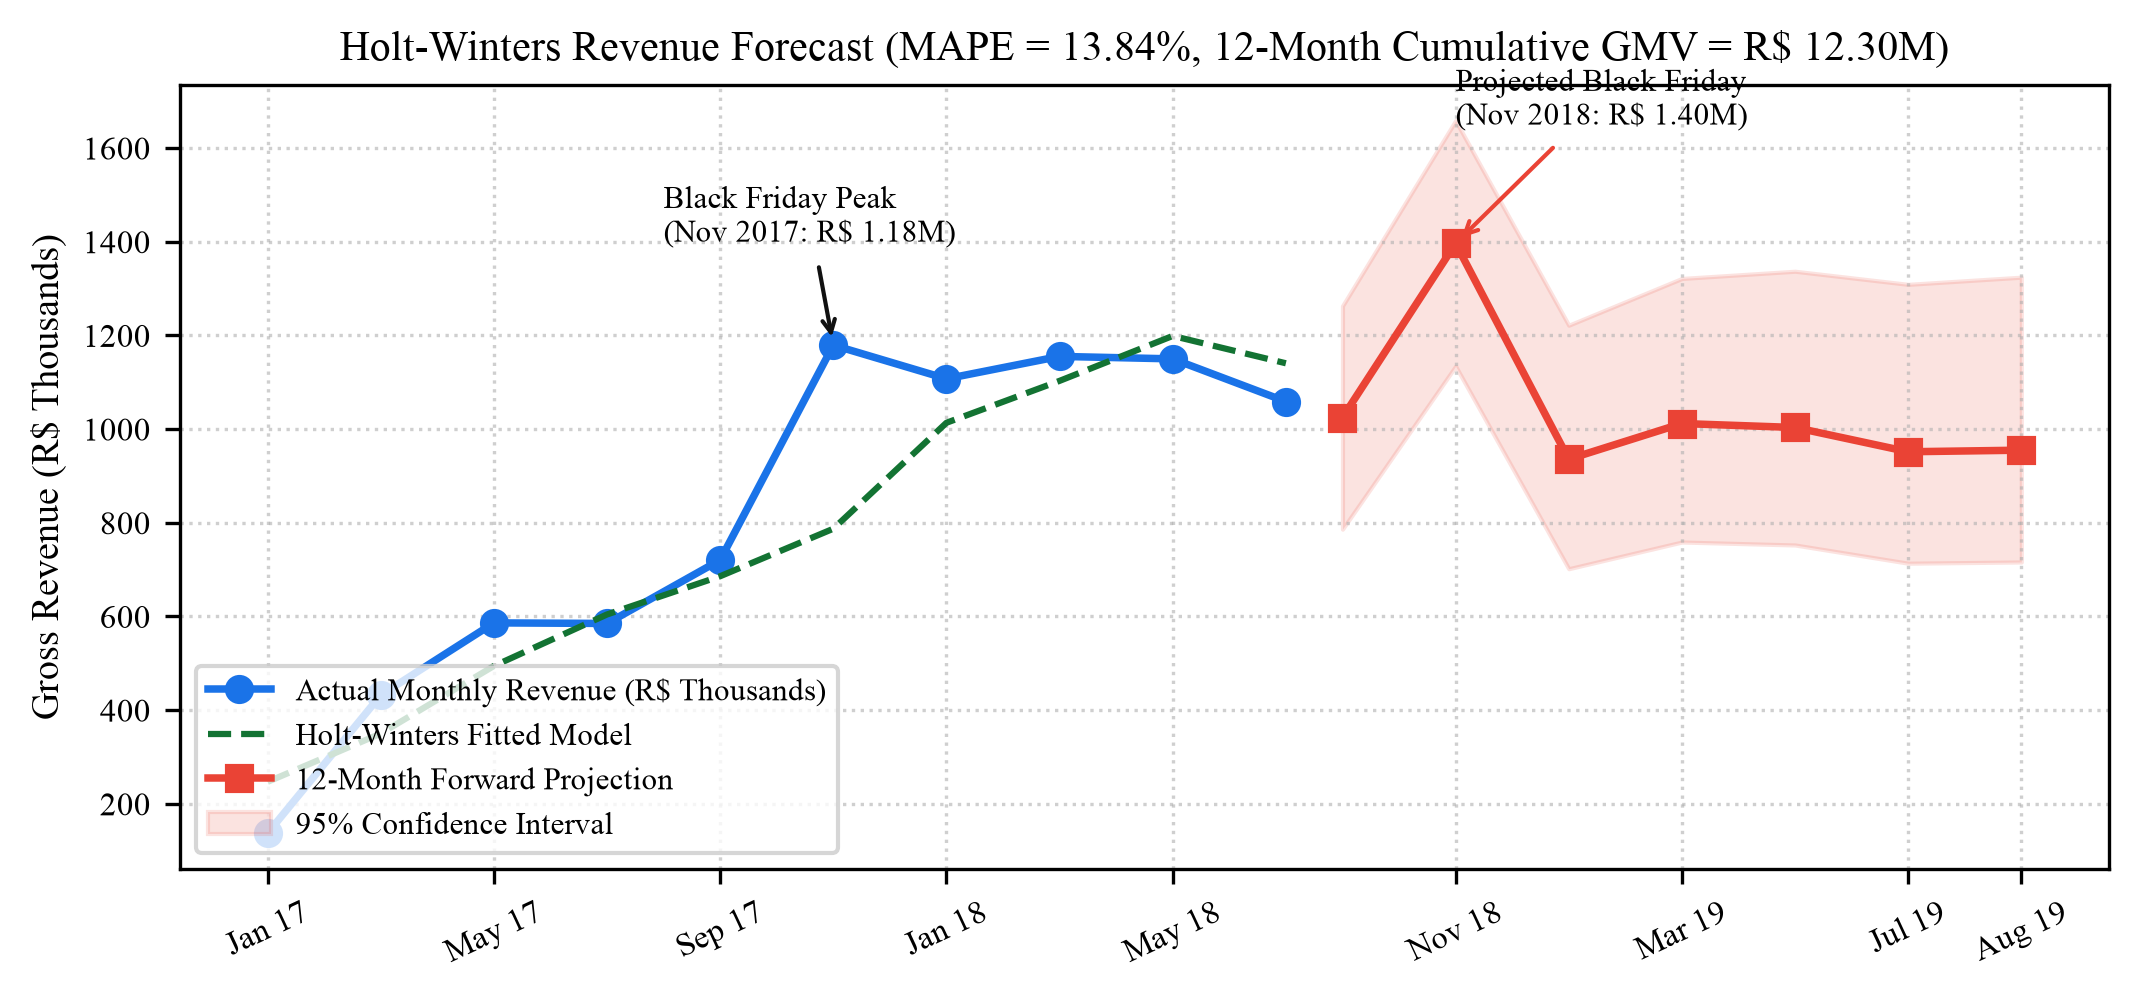
\includegraphics[width=\columnwidth]{figures/fig5_revenue_forecasting.png}
\caption{Historical 20-month monthly revenue fit alongside 12-month forward Holt-Winters projection with 95\% confidence intervals and Black Friday seasonal peaks.}
\label{fig:forecast}
\end{figure}

\subsection{Macro-Regional Logistics and Marketing Attribution}
Empirical breakdown across Brazil's five macro-regions highlights acute geographic disparity (Table III and Fig. 6). While the Southeast drives 64.58\% of platform revenue (R\$ 10.23M) with a 13.14\% freight ratio, the Northern region incurs an \textbf{18.53\%} shipping burden on an average order value of R\$ 223.28, exposing a clear barrier to customer acquisition.

\begin{figure}[htbp]
\centering
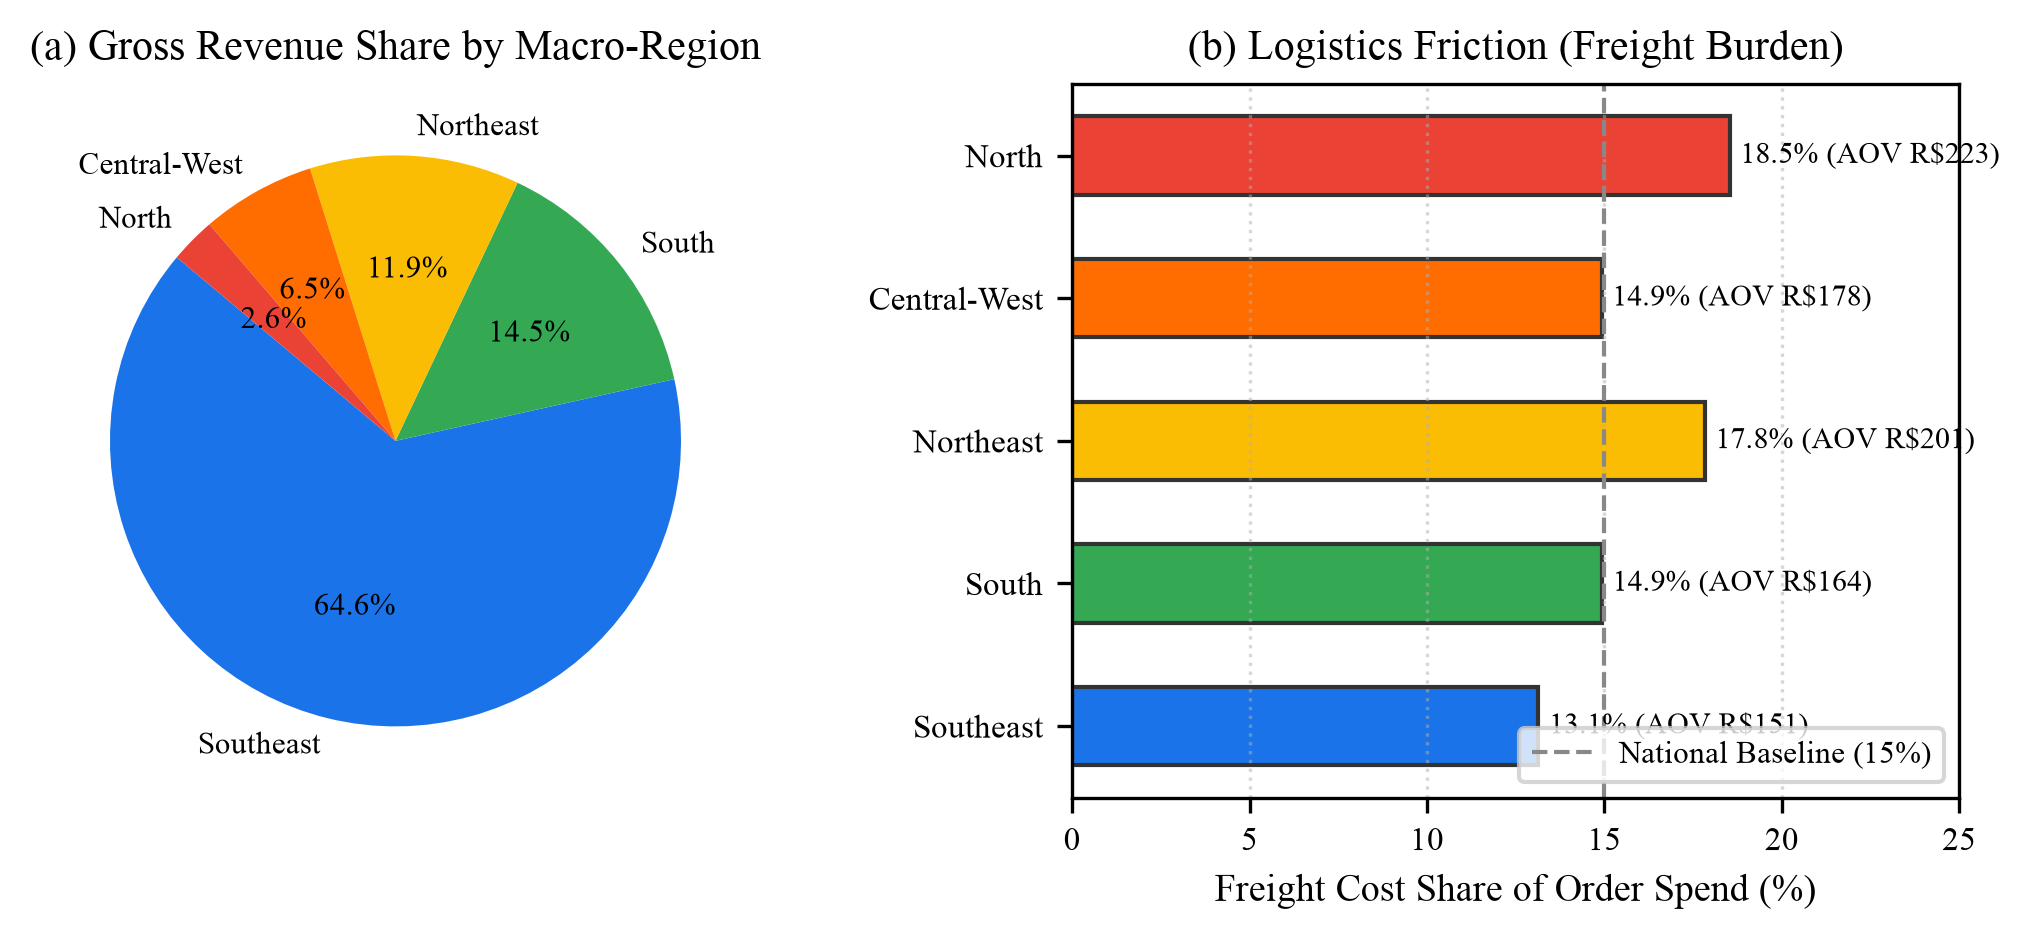
\includegraphics[width=\columnwidth]{figures/fig6_regional_economics.png}
\caption{(a) Regional gross merchandise volume distribution; (b) Logistics friction across Brazilian macro-regions illustrating freight burden disparity.}
\label{fig:regional}
\end{figure}

\begin{table}[h]
\caption{Macro-Regional Revenue and Marketing Attribution}
\label{tab:macro_mktg}
\centering
\resizebox{\columnwidth}{!}{
\begin{tabular}{lcccc}
\toprule
\textbf{Dimension / Entity} & \textbf{Volume} & \textbf{Gross Rev (R\$)} & \textbf{AOV / CAC} & \textbf{ROAS / Freight} \\
\midrule
\textbf{Southeast Region} & 67,706 ord & 10,232,323.50 & R\$ 151.13 & 13.14\% freight \\
\textbf{South Region} & 14,042 ord & 2,296,975.80 & R\$ 163.58 & 14.93\% freight \\
\textbf{Northeast Region} & 9,336 ord & 1,880,799.54 & R\$ 201.46 & 17.83\% freight \\
\textbf{North Region} & 1,838 ord & 410,392.40 & R\$ 223.28 & \textbf{18.53\% freight} \\
\midrule
\multicolumn{5}{c}{\textbf{Marketing Attribution (Total Spend: R\$ 2,124,076.30)}} \\
\midrule
Paid Search & 41,441 ord & 6,991,047.19 & CAC: R\$ 19.68 & ROAS: 8.57$\times$ \\
Paid Social & 35,520 ord & 5,991,159.60 & CAC: R\$ 27.45 & ROAS: 6.14$\times$ \\
\textbf{Email Marketing} & 11,841 ord & 1,998,078.63 & \textbf{CAC: R\$ 7.50} & \textbf{ROAS: 22.50$\times$} \\
Affiliate & 9,867 ord & 1,664,156.47 & CAC: R\$ 24.80 & ROAS: 6.80$\times$ \\
\bottomrule
\end{tabular}
}
\end{table}

In product category profitability, \texttt{health\_beauty} acts as the platform Star (R\$ 1.44M GMV, 34.88\% net margin), while \texttt{perfumery} achieves the highest margin at 38.10\% (Fig. 7).

\begin{figure}[htbp]
\centering
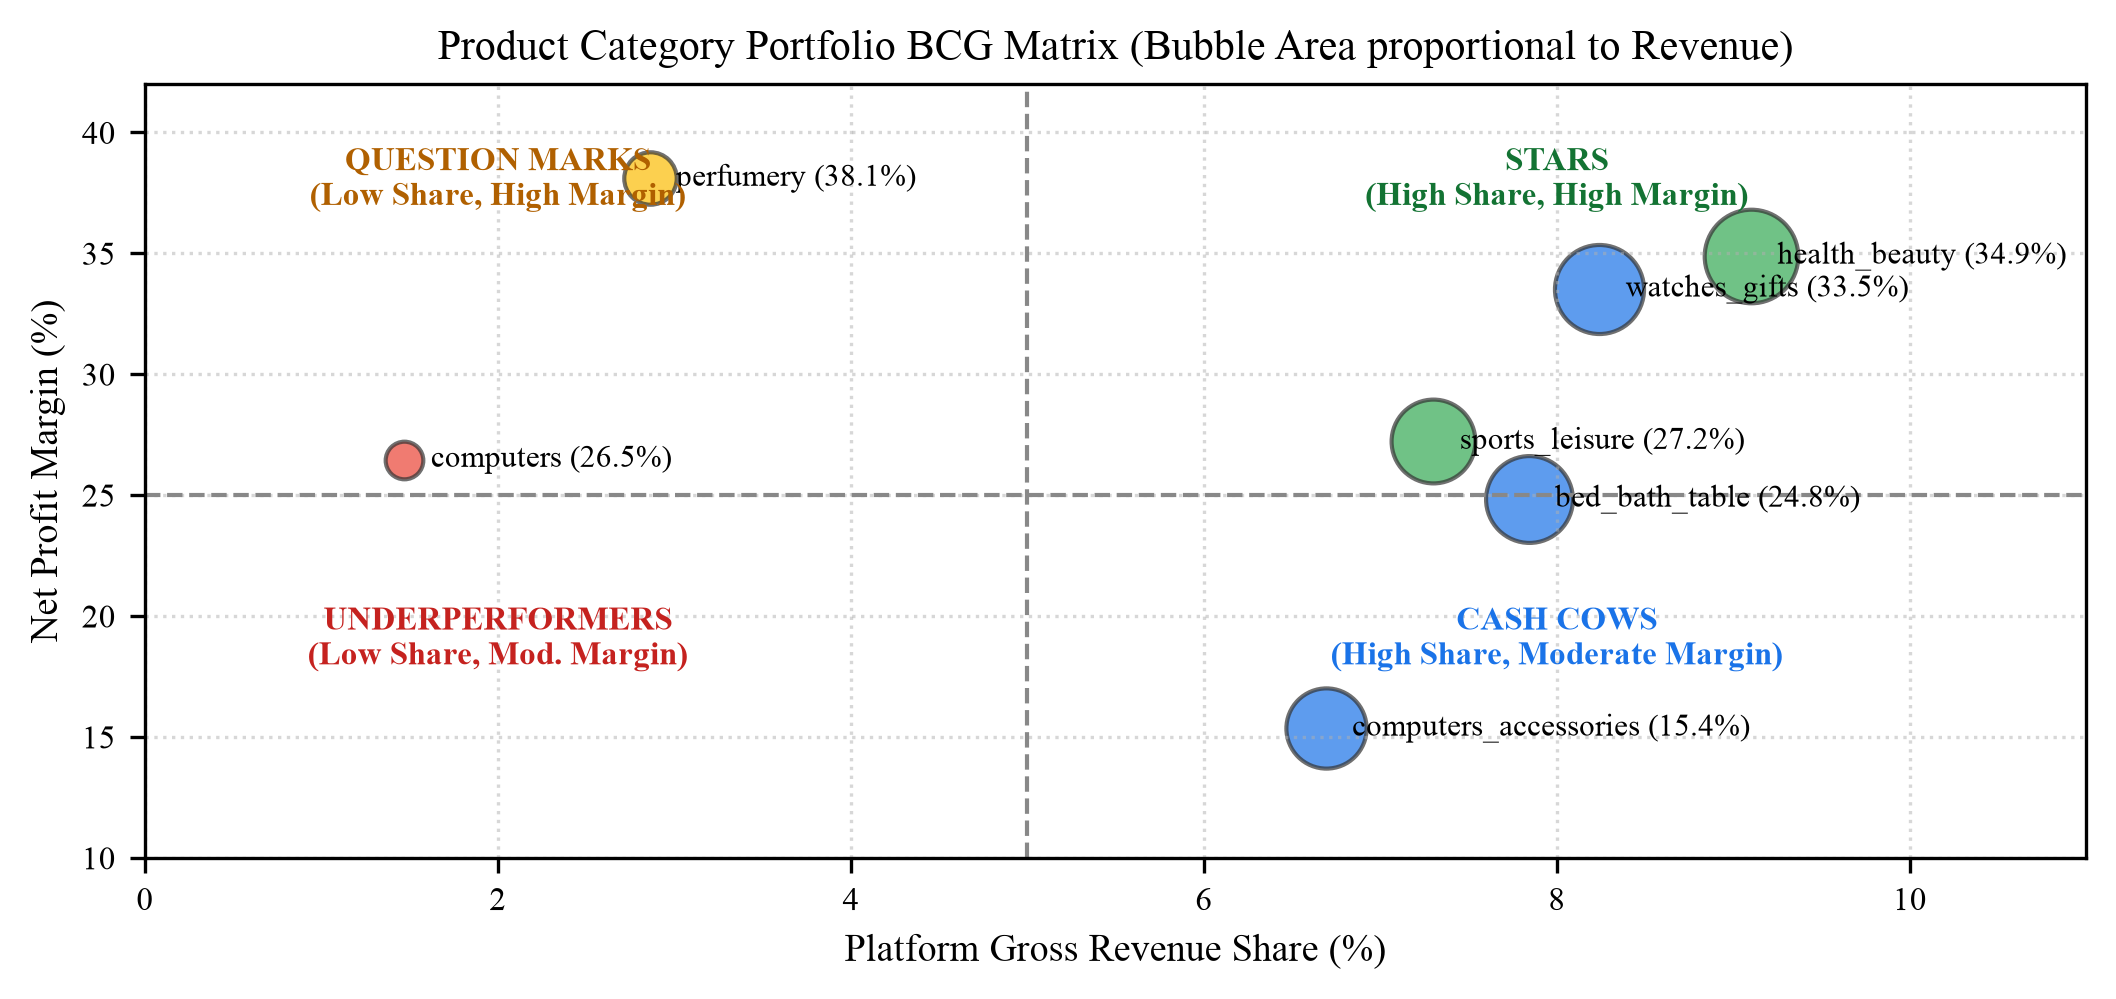
\includegraphics[width=\columnwidth]{figures/fig7_category_bcg_matrix.png}
\caption{Product Category BCG Portfolio Matrix plotting gross revenue share against net margin contribution, with bubble area proportional to absolute revenue.}
\label{fig:bcg}
\end{figure}

\begin{figure}[htbp]
\centering
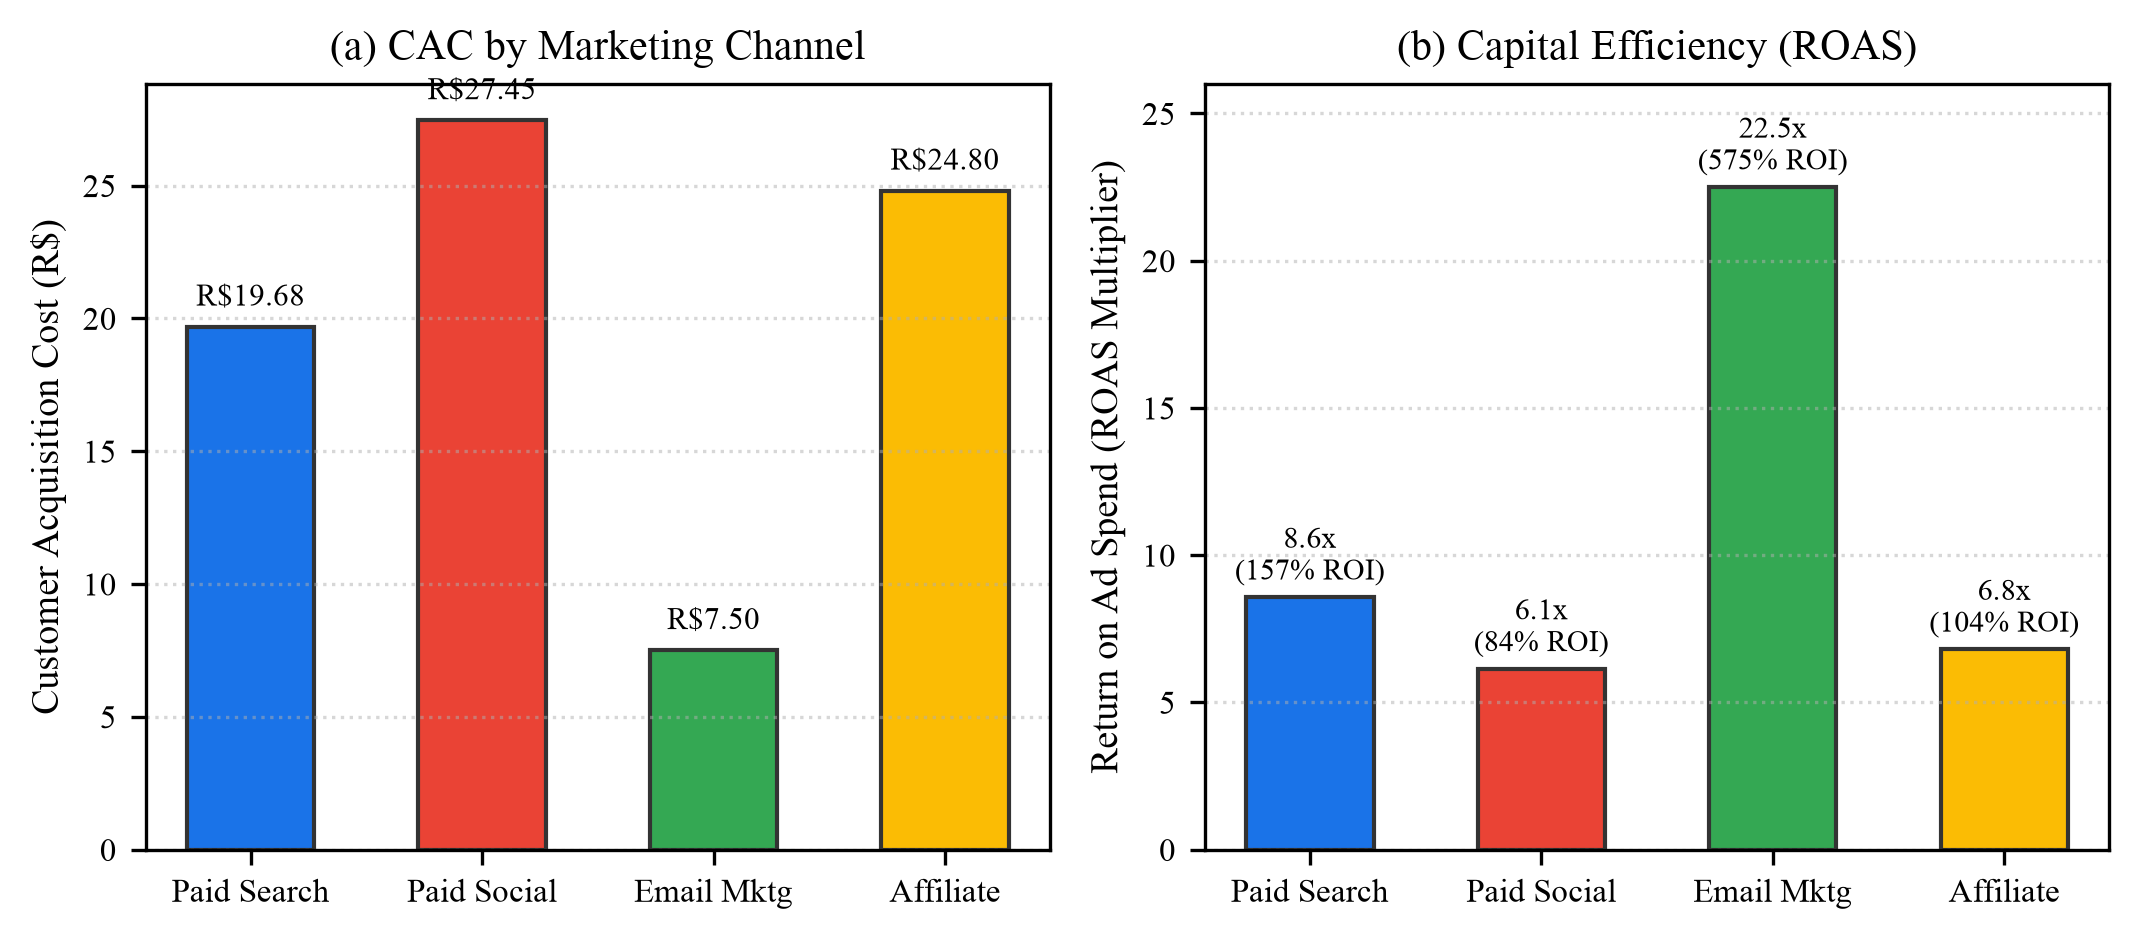
\includegraphics[width=\columnwidth]{figures/fig8_marketing_attribution.png}
\caption{(a) Customer Acquisition Cost (CAC) by channel; (b) Return on Ad Spend (ROAS) and percentage ROI, isolating Email Marketing as the highest-yielding channel.}
\label{fig:mktg}
\end{figure}

In marketing channel efficiency, Email Marketing emerged as the superior capital allocator, producing \textbf{22.50$\times$ ROAS} and \textbf{575\% ROI} at a CAC of only \textbf{R\$ 7.50}, compared to Paid Social's R\$ 27.45 CAC (Fig. 8).

\section{Conclusion and Future Work}
This paper presented \textbf{NEXUS.AI}, a comprehensive enterprise e-commerce intelligence system unifying relational star-schema data warehousing with predictive machine learning and high-availability cloud analytics. The platform demonstrated superior empirical results: 99.28\% churn classification accuracy, actionable 4-persona customer clustering, resilient seasonal revenue forecasting (13.84\% MAPE), and robust dual-mode serverless edge execution on Vercel.

While highly effective, current limitations include the reliance on historical batch snapshots rather than real-time clickstream events, and linear seasonal smoothing during extreme macroeconomic volatility. Future research pathways comprise:
\begin{itemize}
    \item \textbf{Distributed Event Streaming}: Integrating Apache Kafka and Apache Flink for real-time clickstream event processing and real-time dynamic churn scoring.
    \item \textbf{Deep Sentiment Mining}: Deploying transformer-based language models (e.g., BERT/RoBERTa) to automatically extract latent seller defect signals from Portuguese customer review texts.
    \item \textbf{Dynamic Algorithmic Pricing}: Developing multi-armed bandit and reinforcement learning frameworks to optimize localized freight subsidies and promotional discount allocation.
\end{itemize}

\balance
\begin{thebibliography}{00}
\bibitem{kimball2013data} R. Kimball and M. Ross, \textit{The Data Warehouse Toolkit: The Definitive Guide to Dimensional Modeling}, 3rd ed. Hoboken, NJ: John Wiley \& Sons, 2013.
\bibitem{verhoef2002understanding} P. C. Verhoef, ``Understanding the effect of customer relationship management efforts on customer retention and customer share development,'' \textit{Journal of Marketing}, vol. 67, no. 4, pp. 30--45, 2003.
\bibitem{fader2005rfm} P. S. Fader, B. G. Hardie, and K. L. Lee, ``Counting your customers the easy way: An alternative to the Pareto/NBD model,'' \textit{Marketing Science}, vol. 24, no. 2, pp. 275--284, 2005.
\bibitem{chen2016xgboost} T. Chen and C. Guestrin, ``XGBoost: A scalable tree boosting system,'' in \textit{Proc. 22nd ACM SIGKDD Int. Conf. Knowl. Discovery Data Mining}, 2016, pp. 785--794.
\bibitem{gardner1985forecasting} E. S. Gardner Jr, ``Exponential smoothing: The state of the art,'' \textit{Journal of Forecasting}, vol. 4, no. 1, pp. 1--28, 1985.
\bibitem{vafeiadis2015comparison} T. Vafeiadis, K. I. Diamantaras, G. Sarigiannidis, and K. C. Chatzisavvas, ``A comparison of machine learning techniques for customer churn prediction,'' \textit{Simulation Modelling Practice and Theory}, vol. 55, pp. 1--9, 2015.
\bibitem{hartigan1979algorithm} J. A. Hartigan and M. A. Wong, ``Algorithm AS 136: A k-means clustering algorithm,'' \textit{Journal of the Royal Statistical Society. Series C (Applied Statistics)}, vol. 28, no. 1, pp. 100--108, 1979.
\end{thebibliography}

\end{document}
